\section{Design}


\subsection{Framework}
\begin{frame}
\frametitle{Vild titel}
\begin{itemize}
\item Abstrahere væk fra Android platformen
\item Opbygget omkring brug af forskellige \textit{''screens''}
\item Spillet er indeholdt i en aktivitet
\item Til grafik og lyd er der en klasse til hver der eksponerer basale metoder
\item \textit{''Deltatime''} er den tid der går mellem hver frame
\end{itemize}
\end{frame}


\subsection{Kontrol af bil}
\begin{frame}
\frametitle{Det gamle Cars}
\begin{itemize}
\item Kontrol af bilen var baseret på frekvens(mere om det her måske???)
\item Det var svært at styre, hvis ikke umuligt
\end{itemize}
\end{frame}

\begin{frame}
\frametitle{Sprint 2}
\begin{itemize}
\item Skiftet fra frekvens til volumen
\item Krav: \textit{The car is controlled in such a way,
that the vertical position of the car is relative
to the current loudness of the player's voice.}
\end{itemize}
\begin{figure}
\centering
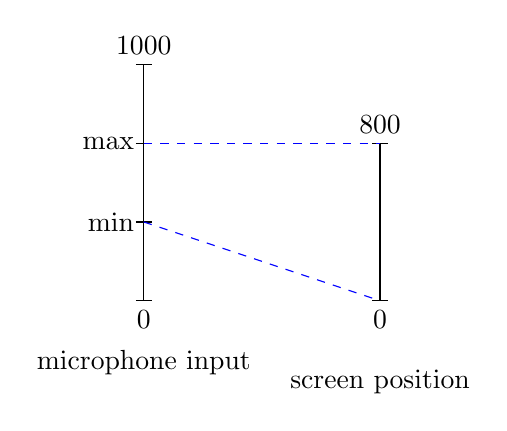
\begin{tikzpicture}
%vertical scales
\draw (0,0) -- (0,3); 
\draw (3,0) -- (3,2);

\node [below] at (0,-0.5){microphone input};
\node [below] at (3,-0.75){screen position};

%  endpoints with labels
\draw (-0.1,0) -- (0.1,0); 
\node [below] at (0,0){0};

\draw (-0.1,3) -- (0.1,3);
\node [above] at (0,3){1000};

\draw (2.9,0) -- (3.1,0); 
\node [below] at (3,0){0};

\draw (2.9,2) -- (3.1,2);
\node [above] at (3,2){800};

%min and max labels 
\draw (-0.1,1) -- (0.1,1);
\node [left] at (0,1){min};

\draw (-0.1,2) -- (0.1,2);
\node [left] at (0,2){max};

% mapping lines
\draw [dashed, blue](0,2) -- (3,2);
\draw [dashed, blue](0,1) -- (3,0);
\end{tikzpicture}
\caption{The mapping from microphone input to position on the screen}
\end{figure}
\end{frame}

\begin{frame}
\frametitle{Sprint 3}
\begin{itemize}
\item Stabilisering af bilen
\item Forskellige afprøvede metoder:
\begin{itemize}
\item Linær bevægelse(???)
\item Gennemsnit
\item Acceleration og deceleration (Valgt)
\end{itemize}
\end{itemize}
\end{frame}


\subsection{Kalibrering}
\begin{frame}
\frametitle{title--}
\begin{itemize}
\item Krav: \textit{It must be possible to calibrate the microphone}
\item Kalibreringen sætter en max og en min værdi
\item Projektets problembarn
\item Den grafiske fremstilling i indstillinger var meget udfordrende
\end{itemize}
\end{frame}

\begin{frame}
\frametitle{Visuelle udvikling for kalibrering(vildeste titel.--")}
\begin{figure}
\begin{subfigure}[b]{0.4\textwidth}
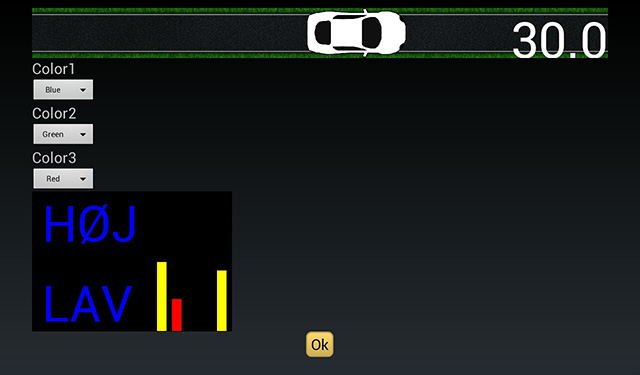
\includegraphics[width=130px]{sprint2/settings}
\caption{The settings activity from sprint 2}
\end{subfigure}
~
\begin{subfigure}[b]{0.4\textwidth}
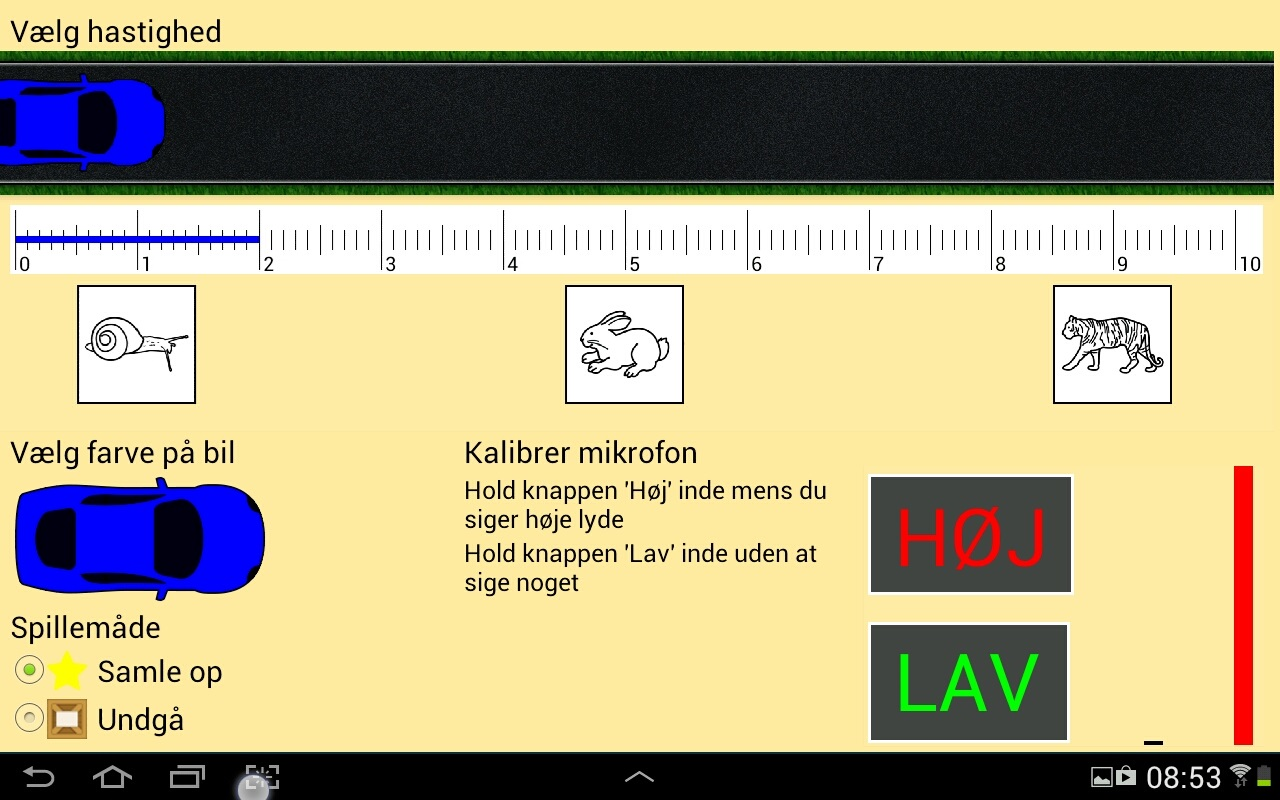
\includegraphics[width=130px]{sprint4/settings_s4}
\caption{The settings activity from sprint 4}
\end{subfigure}
\end{figure}
\end{frame}

\subsection{Mål med spillet}
\begin{frame}
\frametitle{Gamle Cars}
Undgå forskellige forhindringer og køre i den garage som har den samme farve som bilen
\begin{figure}
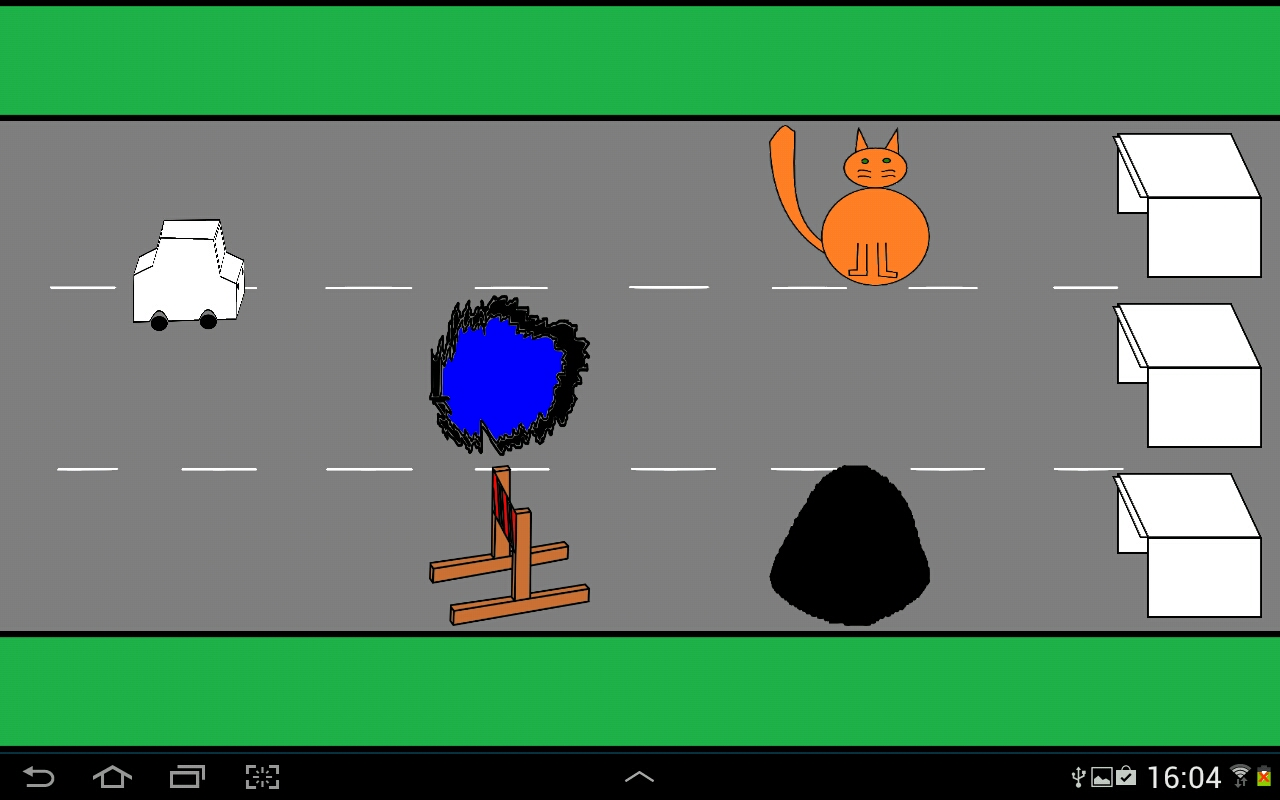
\includegraphics[width=130px]{sprint1/cars_screenshot}
\caption{The old cars}
\end{figure}
\end{frame}

\begin{frame}
\frametitle{Nuværende Cars}
\begin{itemize}
\item Krav sprint 2: \textit{The goal of the game is to reach a garage}
\item Krav sprint 4: \textit{The goal of the game is to reach the finishing line
after successfully collecting all items or avoiding
all items (two different game modes)}
\end{itemize}
\begin{figure}
\begin{subfigure}[b]{0.4\textwidth}
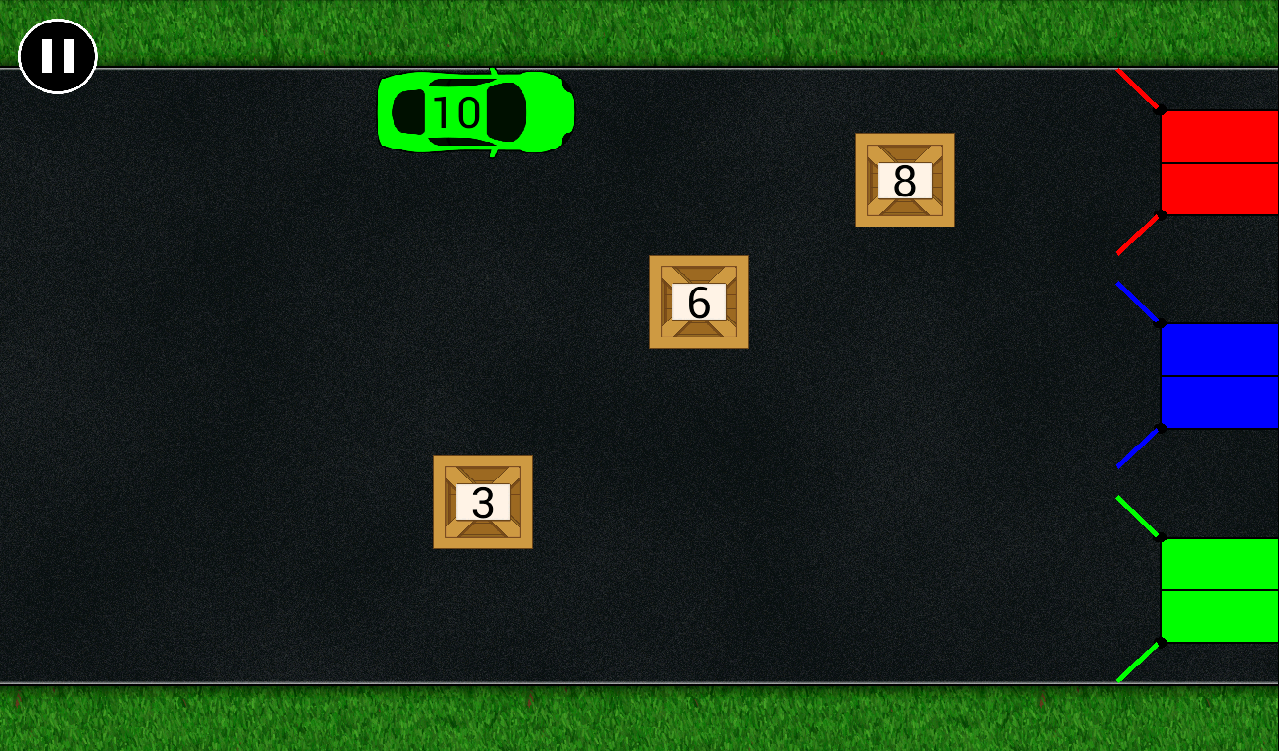
\includegraphics[width=125px]{sprint2/sound_gauge}
\caption{Sprint 2}
\end{subfigure}
~
\begin{subfigure}[b]{0.4\textwidth}
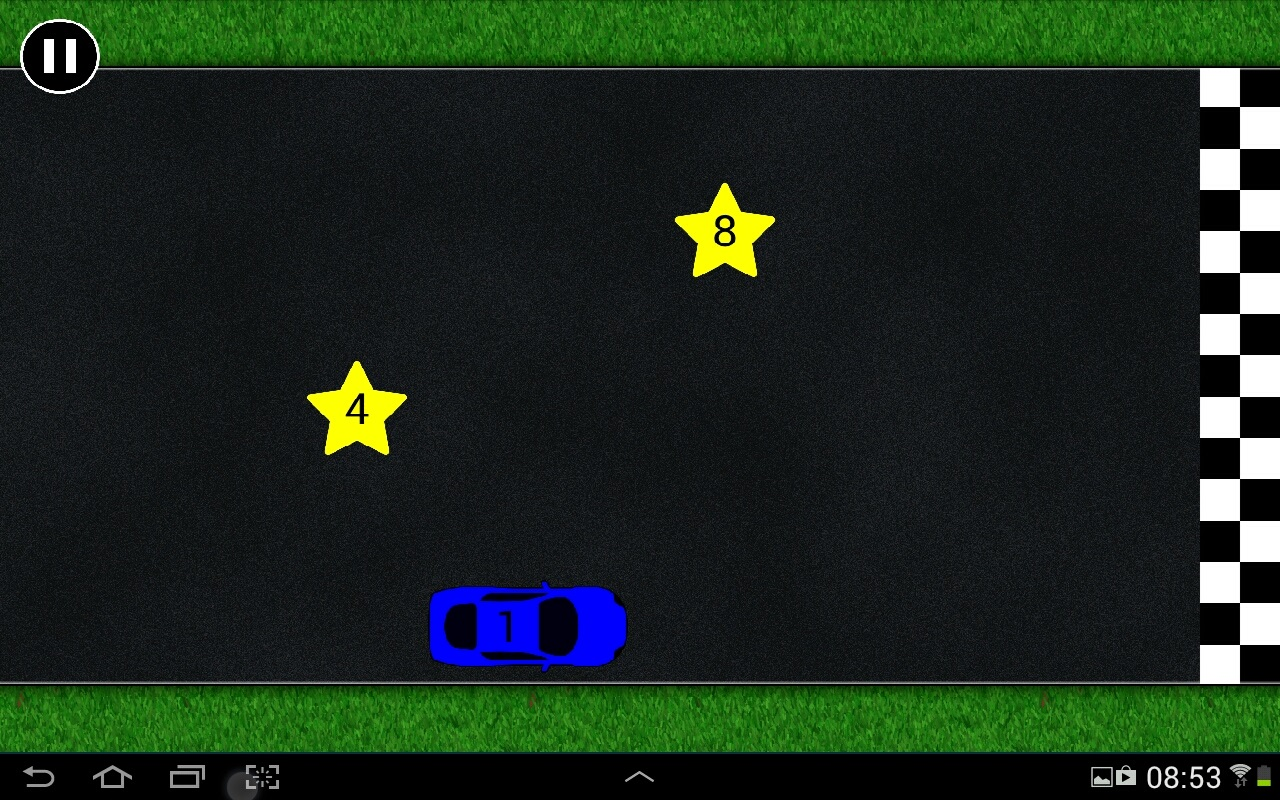
\includegraphics[width=125px]{sprint4/game}
\caption{Sprint 4}
\end{subfigure}
\end{figure}
\end{frame}
\subsection{GUI}
\begin{frame}
\frametitle{Bane og settings}
synes jeg ikke er nødvendig når vi har goal of the game, barometre og kalibrering..
\end{frame}
\begin{frame}
\frametitle{Barometre}
\begin{figure}[h]
	\centering
        \begin{subfigure}[b]{0.4\textwidth}
                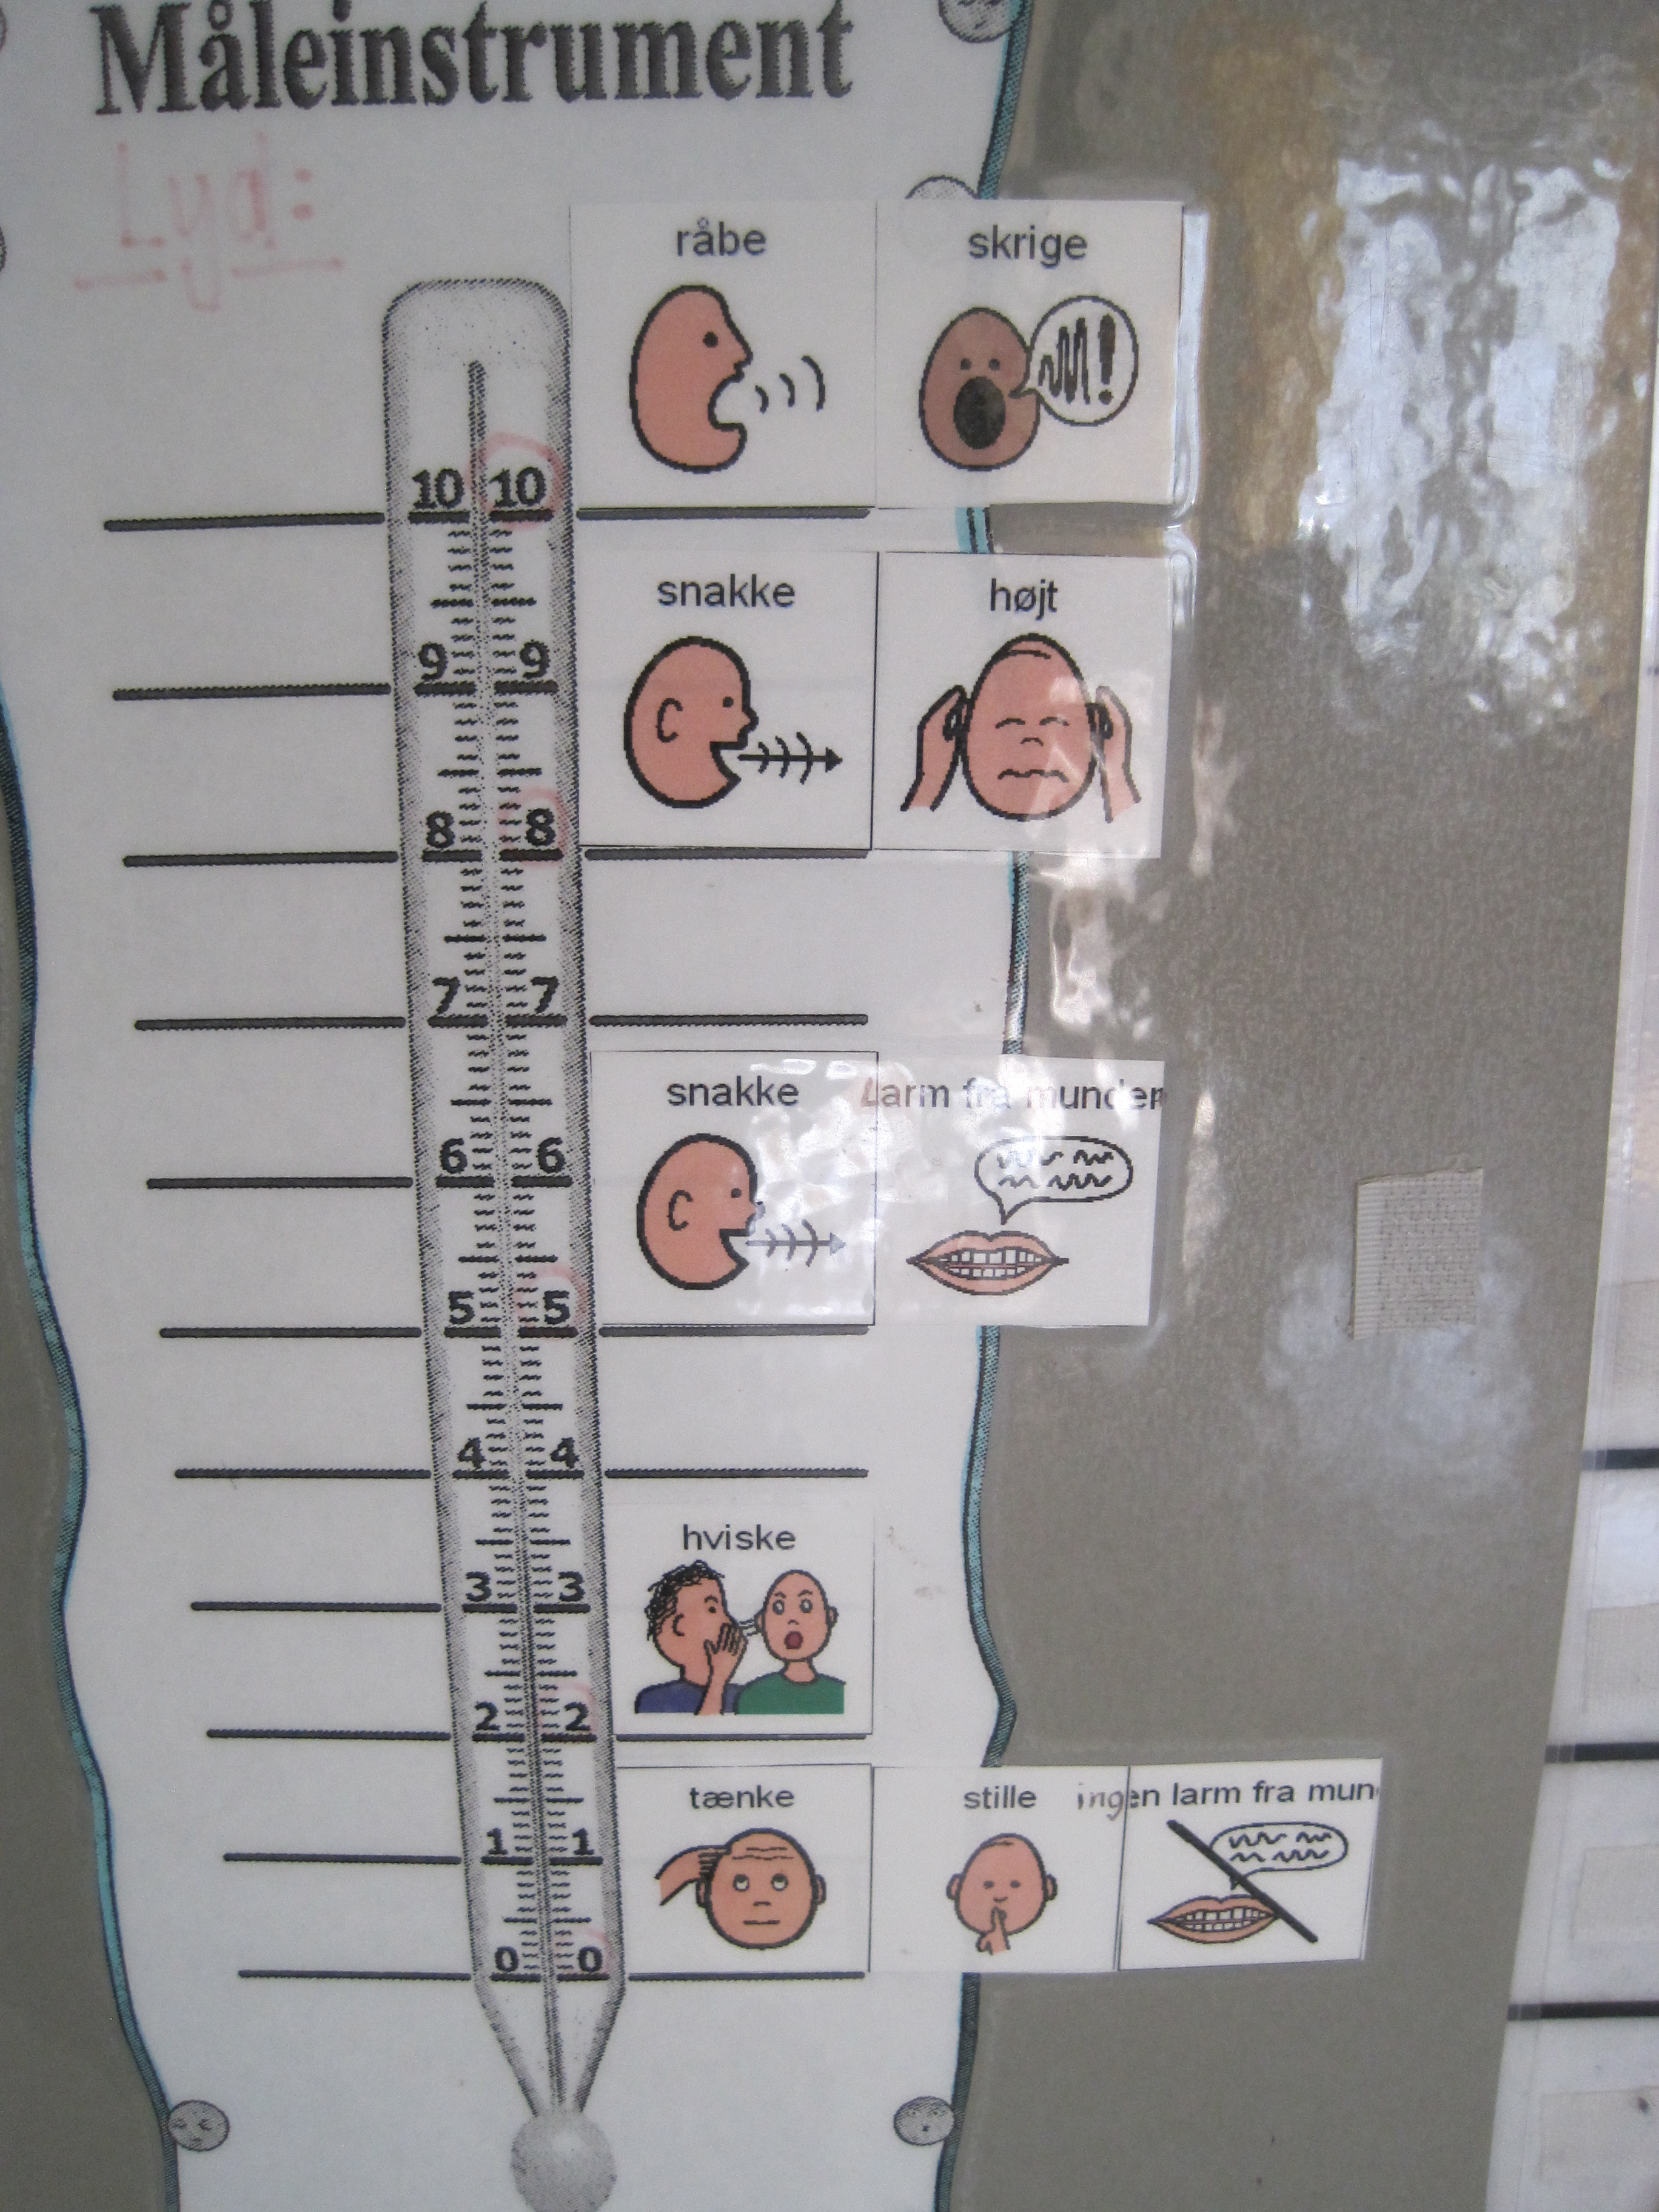
\includegraphics[width=\textwidth]{sprint2/sound}
                \caption{Lydbarometer}
        \end{subfigure}%
        ~
        \begin{subfigure}[b]{0.4\textwidth}
                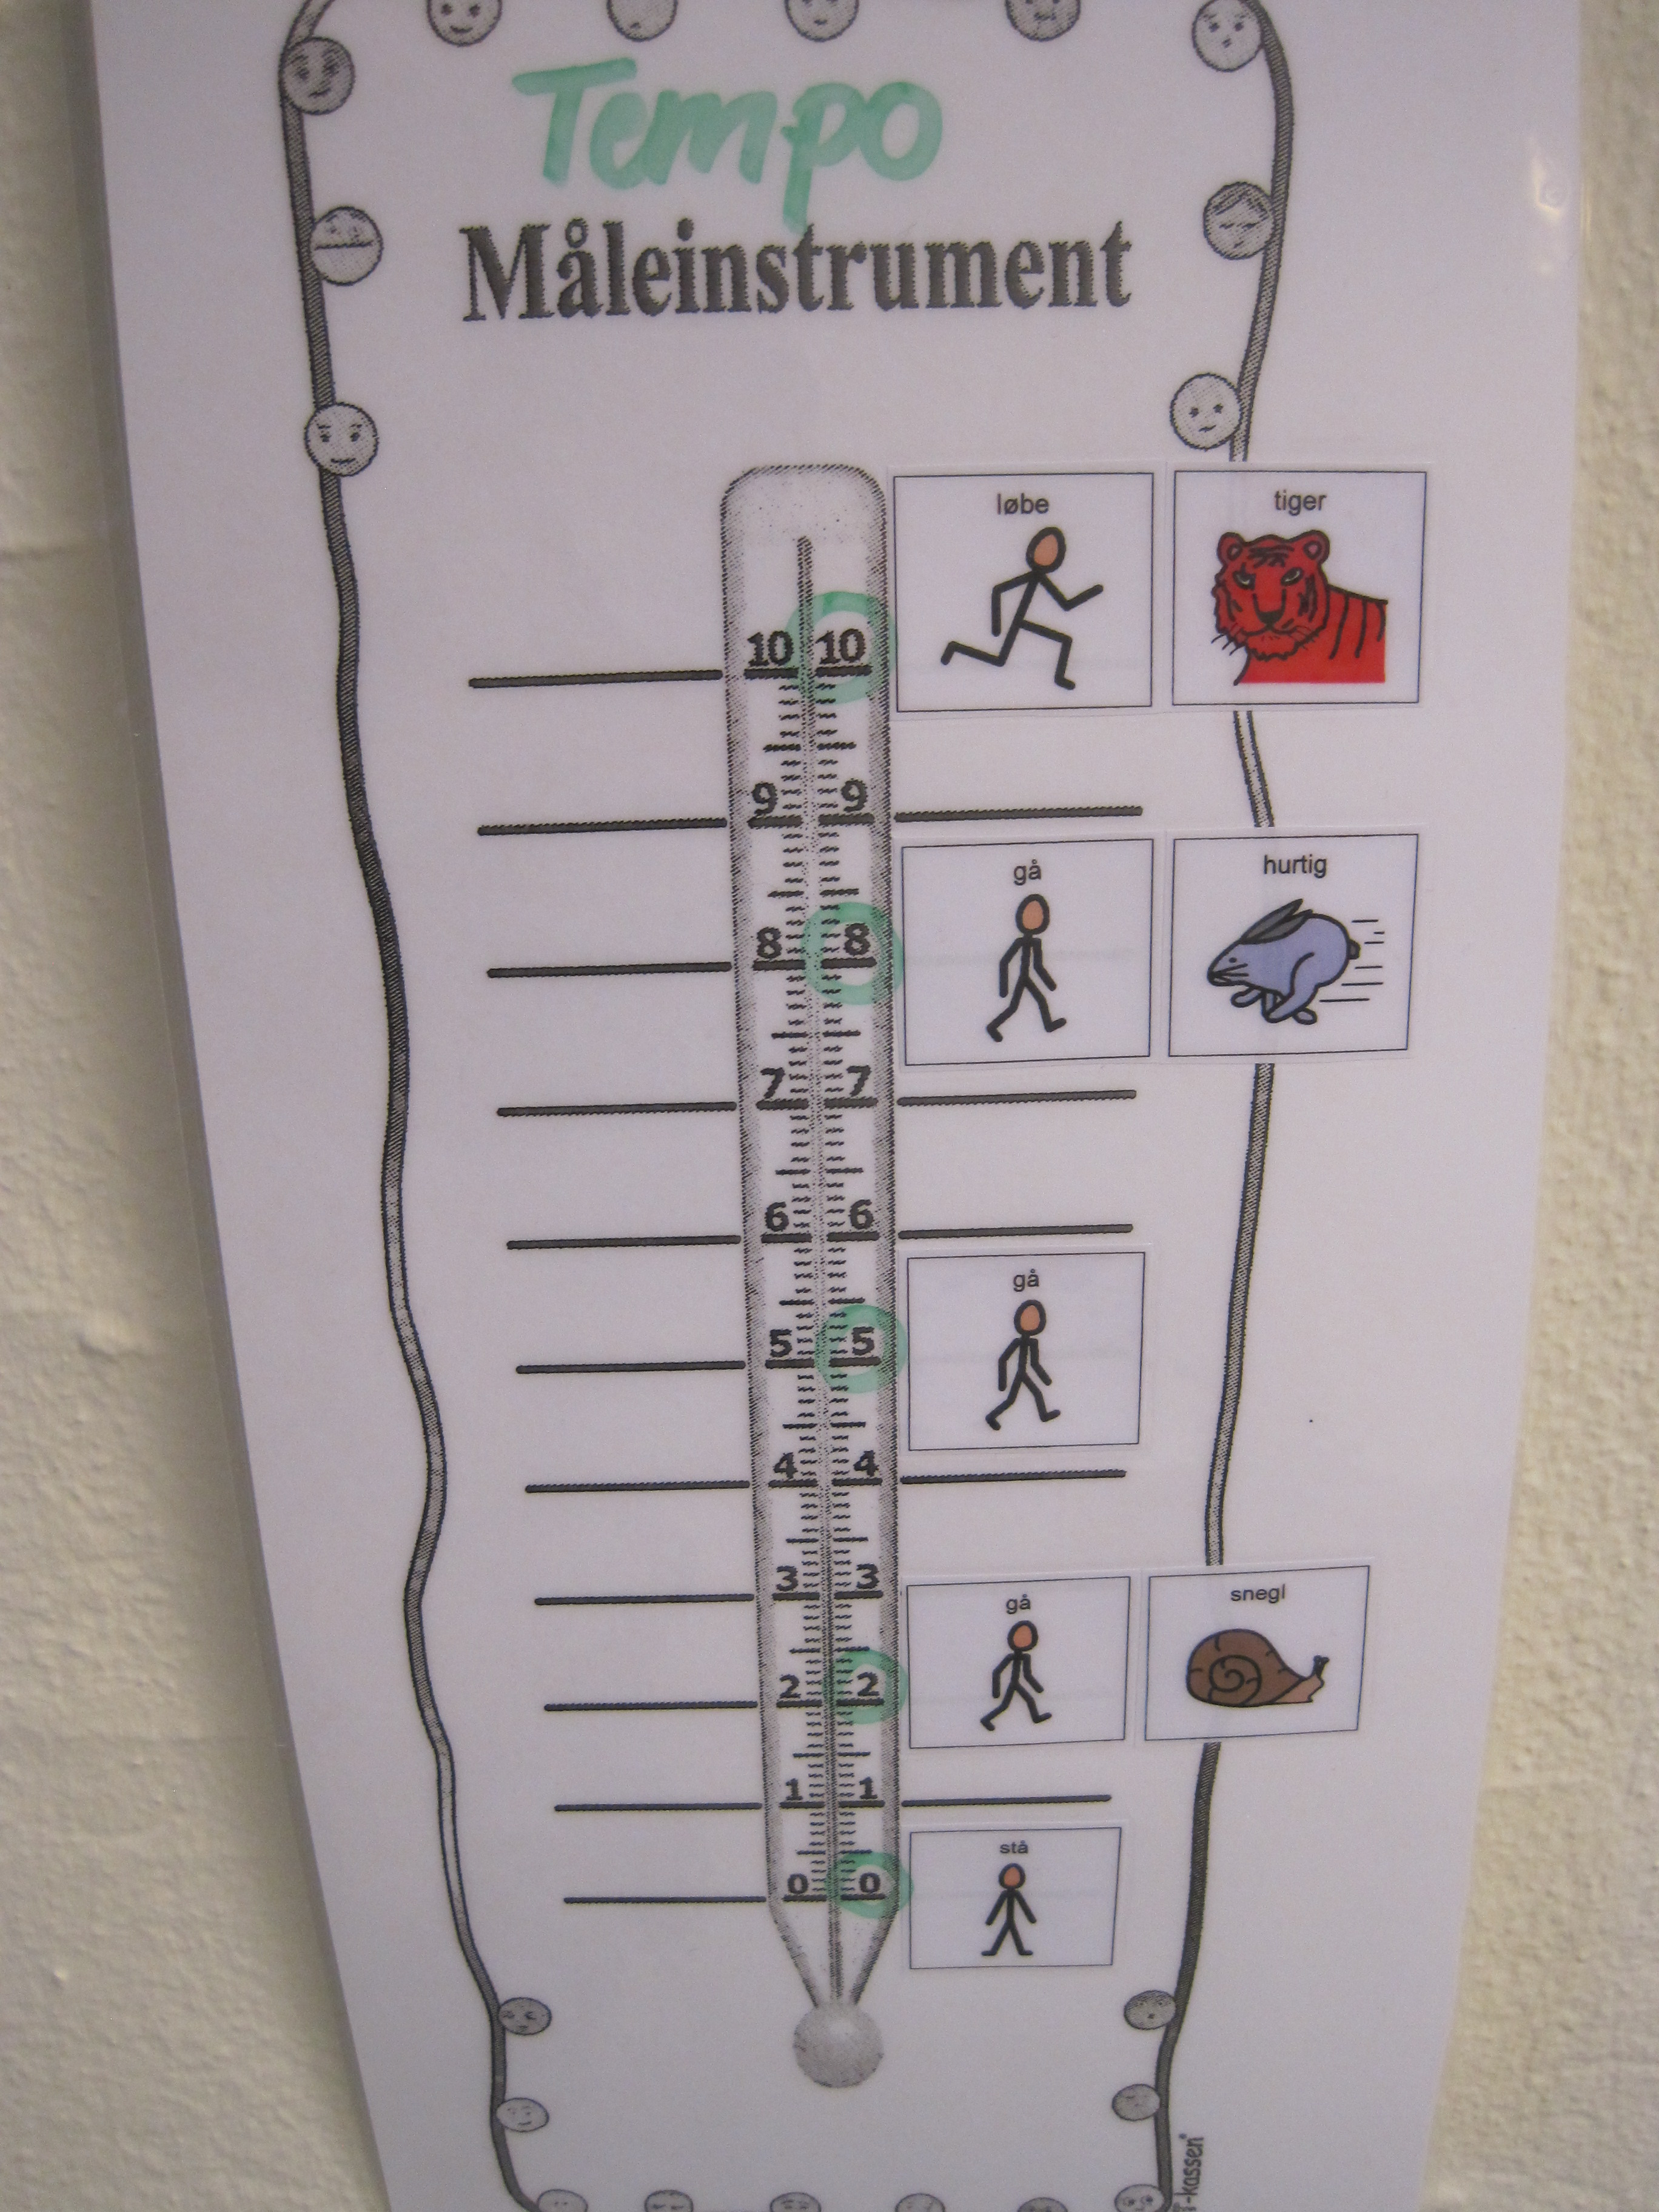
\includegraphics[width=\textwidth]{sprint2/speed}
                \caption{Hastighedsbarometer}
        \end{subfigure}
        \caption{Barometre brugt i 'Birken'}
\end{figure}
\end{frame}

\begin{frame}
\frametitle{Barometre}
\begin{itemize}
\item Krav omkring at inkorporere disse barometre i spillet
\item Tal mellem 0 og 10 på bil, forhindringer og stjerner
\item Mulighed for at pause spillet og se hvor man er henne på barometret
\item Vælge hastighed ud fra et barometer
\end{itemize}
\end{frame}

\begin{frame}
\frametitle{Barometre}
\begin{figure}
\begin{subfigure}[b]{0.4\textwidth}
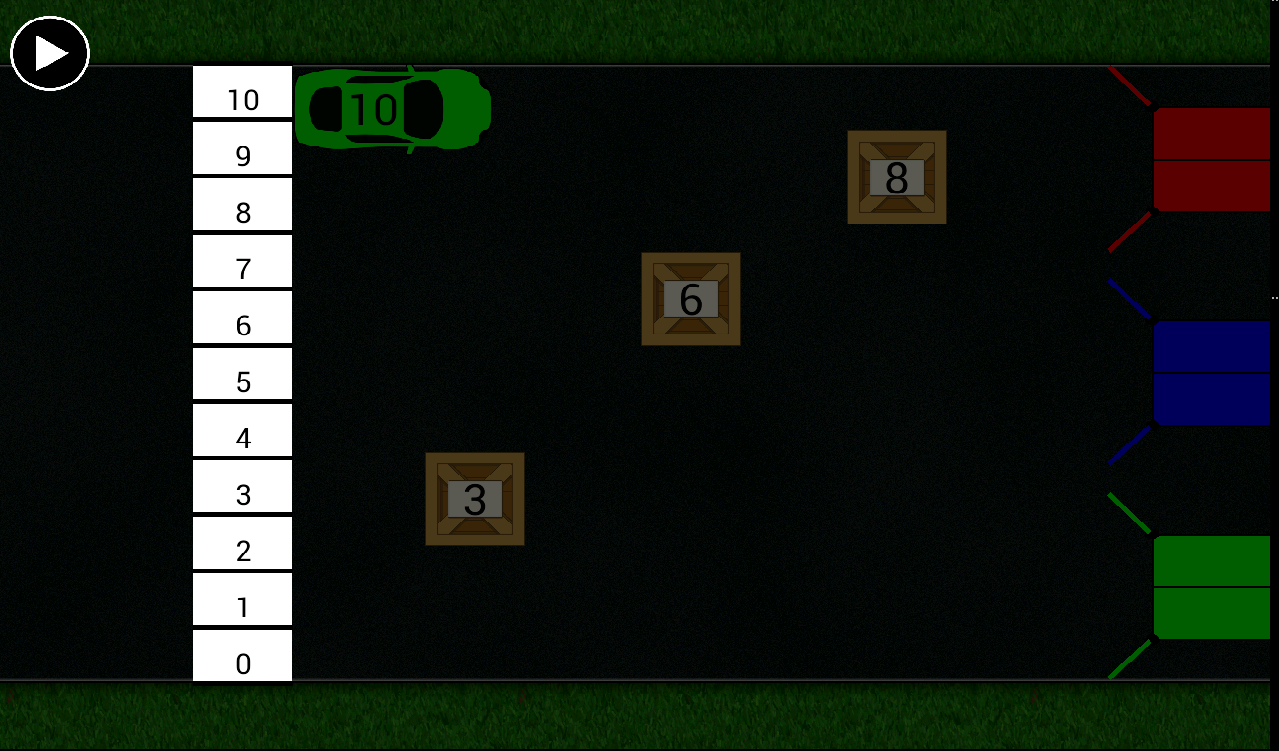
\includegraphics[width=130px]{sprint2/pause}
\caption{The settings activity from sprint 2}
\end{subfigure}
~
\begin{subfigure}[b]{0.4\textwidth}
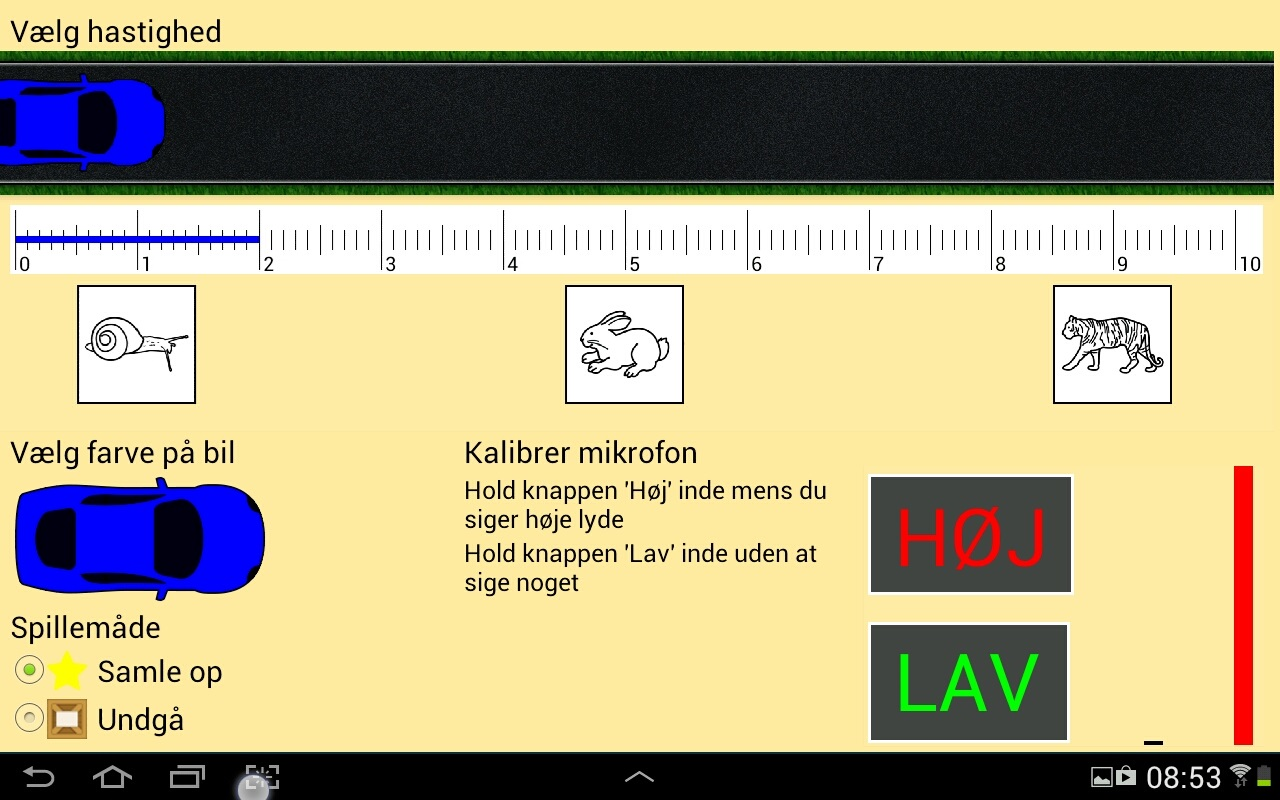
\includegraphics[width=130px]{sprint4/settings_s4}
\caption{The settings activity from sprint 4}
\end{subfigure}
\end{figure}
\end{frame}